\documentclass[11pt]{standalone}
\usepackage{microtype}
\usepackage{tikz}
\author{Phineas Greene}

\SetTracking
 [spacing = {500*,-100*, },]
 { encoding = * }
 { 160 }
 
\begin{document}

\resizebox{1\textwidth}{!}{
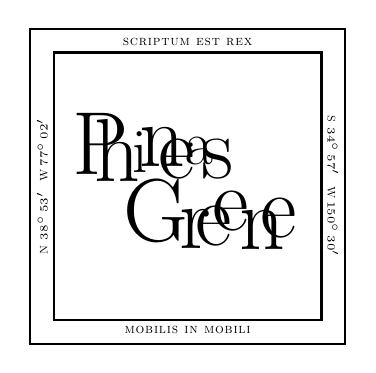
\begin{tikzpicture}[scale=1, every node/.style={transform shape}]

\draw [thick] (0, 0) rectangle (4, 4);

\draw [thick] (0.3, 3.7) -- (2, 3.7) node [above=-1.3pt] {\tiny\textsc{\textls{scriptum est rex}}} -- (3.7, 3.7) -- (3.7, 2) node [right=-1.5pt, anchor=south, rotate=-90, align=center] 
{\scalebox{0.8}{\tiny{\textsc{S} $34^{\circ} \thinspace 57' \thinspace\thinspace$ \textsc{W} $\negthinspace150^{\circ} \thinspace 30'$}}} --
(3.7, 0.3) -- (2, 0.3) node [below=-1.3pt] {\tiny{\textsc{\textls{mobilis in mobili}}}} --
(0.3, 0.3) -- (0.3, 2) node [left=-1.5pt, anchor=south, rotate=90, align=center] 
{\scalebox{0.8}{\tiny{\textsc{N} $38^{\circ} \thinspace 53' \thinspace\thinspace$ \textsc{W} $ \negthinspace 77^{\circ} \thinspace 02'$}}} -- cycle;

\node [text width=1.4in,align=center] at (2, 2) {\hspace{-0.45in}\vspace{-0.02in}
\scalebox{1.3}{
\Huge{\hspace{0ex}\raisebox{-0.1ex}{P}}%
%
\Huge{\hspace{-0.9ex}\raisebox{-0.3ex}{h}}%
%
\LARGE{\hspace{-0.3ex}\raisebox{-0.1ex}{i}}%
%
\Huge{\hspace{-0.2ex}\raisebox{0.1ex}{n}}%
%
\Huge{\hspace{-0.7ex}\raisebox{-0.2ex}{e}}%
%
\LARGE{\hspace{-0.4ex}\raisebox{0.2ex}{a}}%
%
\Huge{\hspace{-0.3ex}\raisebox{-0.2ex}{s}}}%

\hspace{0.12in}
\vspace{0.05in}
\scalebox{1.3}{
\Huge{\hspace{0ex}\raisebox{-0.1ex}{G}}%
%
\Huge{\hspace{-0.25ex}\raisebox{-0.27ex}{r}}%
%
\Huge{\hspace{-0.4ex}\raisebox{-0.2ex}{e}}%
%
\Huge{\hspace{-0.5ex}\raisebox{0.2ex}{e}}%
%
\Huge{\hspace{-0.25ex}\raisebox{-0.3ex}{n}}%
%
\Huge{\hspace{-0.65ex}\raisebox{0ex}{e}}}};
\end{tikzpicture}
}

\end{document}